\documentclass[11pt]{amsart}
\usepackage{amsmath,amsthm,amssymb,amsfonts,epic,epsfig,latexsym,enumerate}
\usepackage{enumitem}
\usepackage[titlenotnumbered,linesnumbered,noend,plain]{algorithm2e}
\usepackage{listings}
\usepackage{fullpage}
\usepackage{setspace}
\usepackage{mathtools}
\usepackage{qtree}
\usepackage{tikz}
\thispagestyle{empty}
\DeclarePairedDelimiter\ceil{\lceil}{\rceil}
\DeclarePairedDelimiter\floor{\lfloor}{\rfloor}

\SetKwProg{Fn}{}{}{}

\newtheorem{lemma}{Lemma}
\usepackage{url}

\SetKwProg{Fn}{}{}{}

\parindent 0cm
\thispagestyle{empty}

\begin{document}

\title{Com S 311 Exam 2}
\author{Nathan Tucker (njtucker@iastate.edu)}
\maketitle

\doublespacing

\vspace{10mm}

\vfill
\begin{flushright}
This assignment represents my own work in accordance with University regulations.

- Nathan Tucker
\end{flushright}
\newpage
\vspace{-.8cm}

\newpage
\hrulefill \\

\textbf{Problem 1:} (Minimum Spanning Trees)\hfill (20 Points)\\

(a) Construct a minimum spanning tree for the graph below on the left. Draw the tree by adding edges to the graph on the right.

\begin{figure}[htb]
\begin{center}
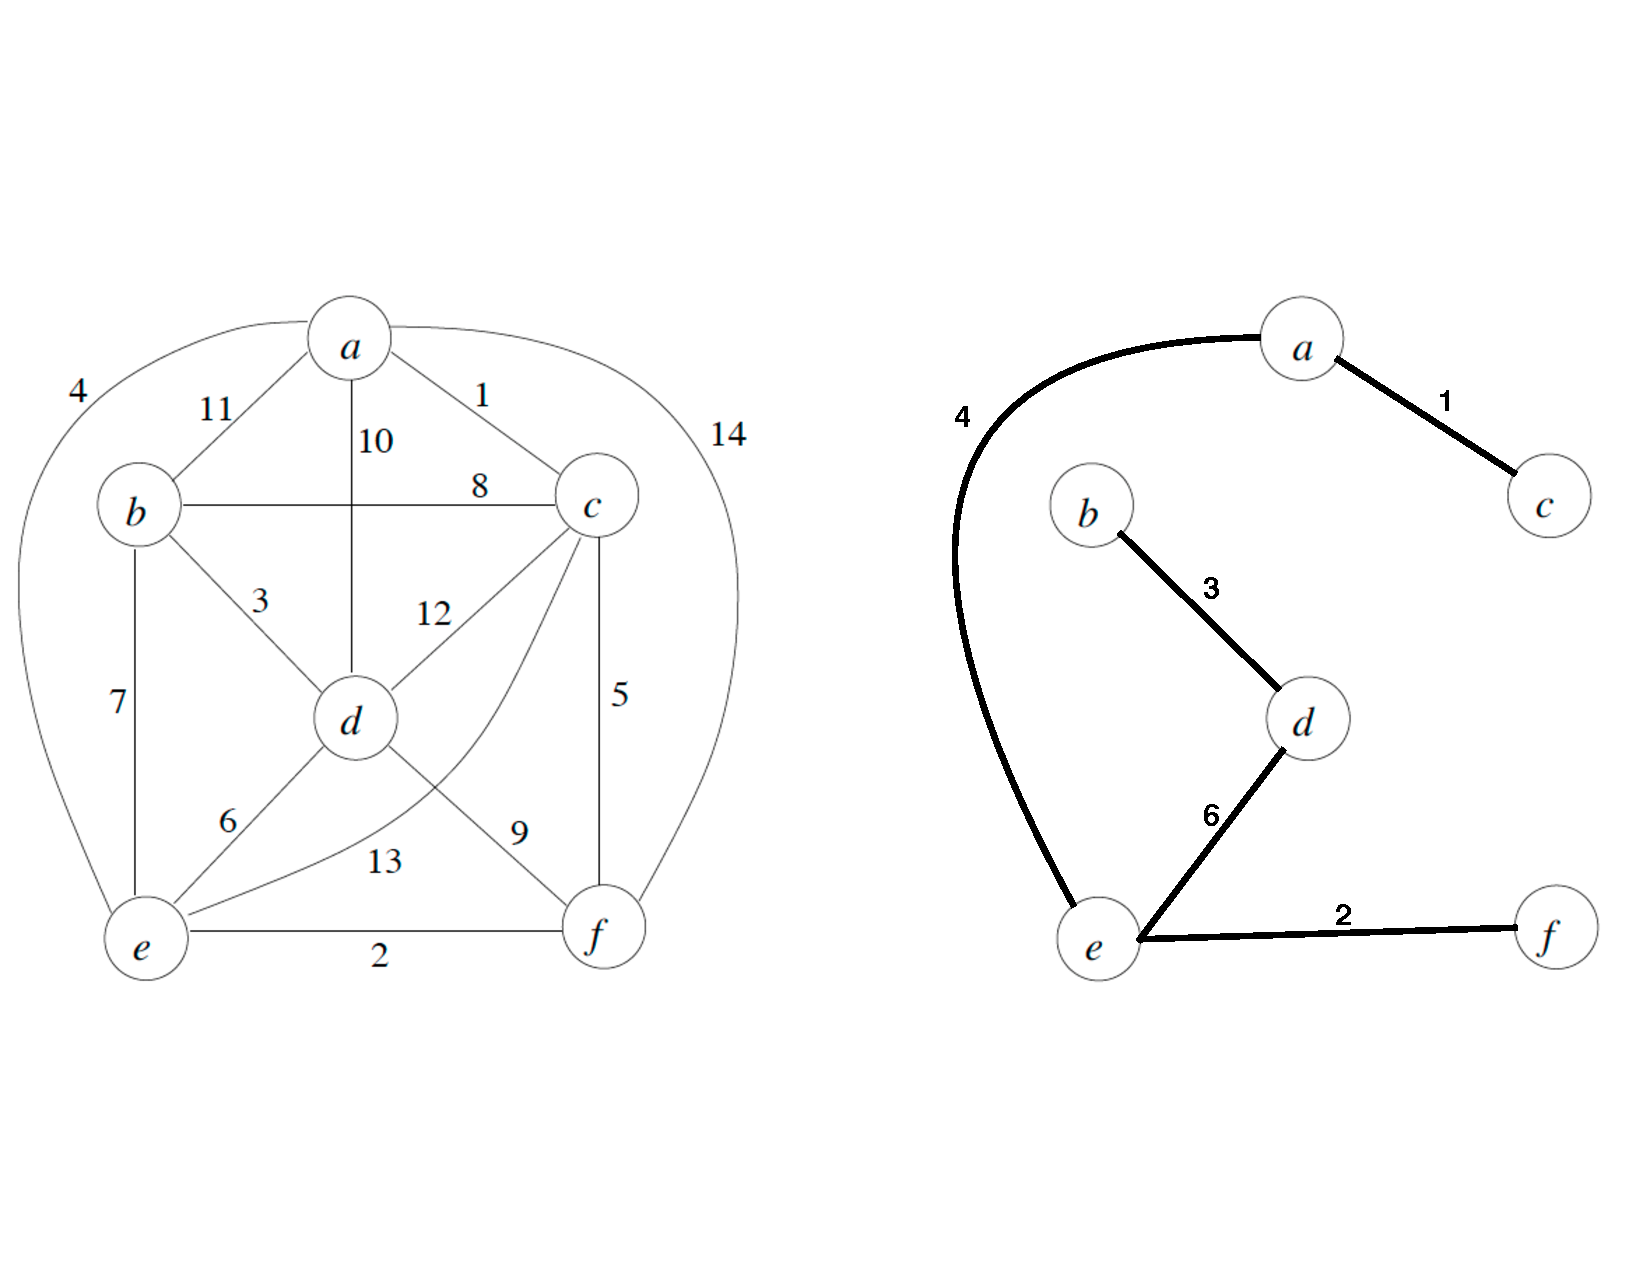
\includegraphics[width=\textwidth]{MSTf.pdf}
\end{center}
\end{figure}

(b) Fill out the table below with the edges of the above minimum spanning tree according to their orders of selection by Kruskal's 
and Prim's algorithms, respectively.

\begin{figure}[htb]
\begin{center}
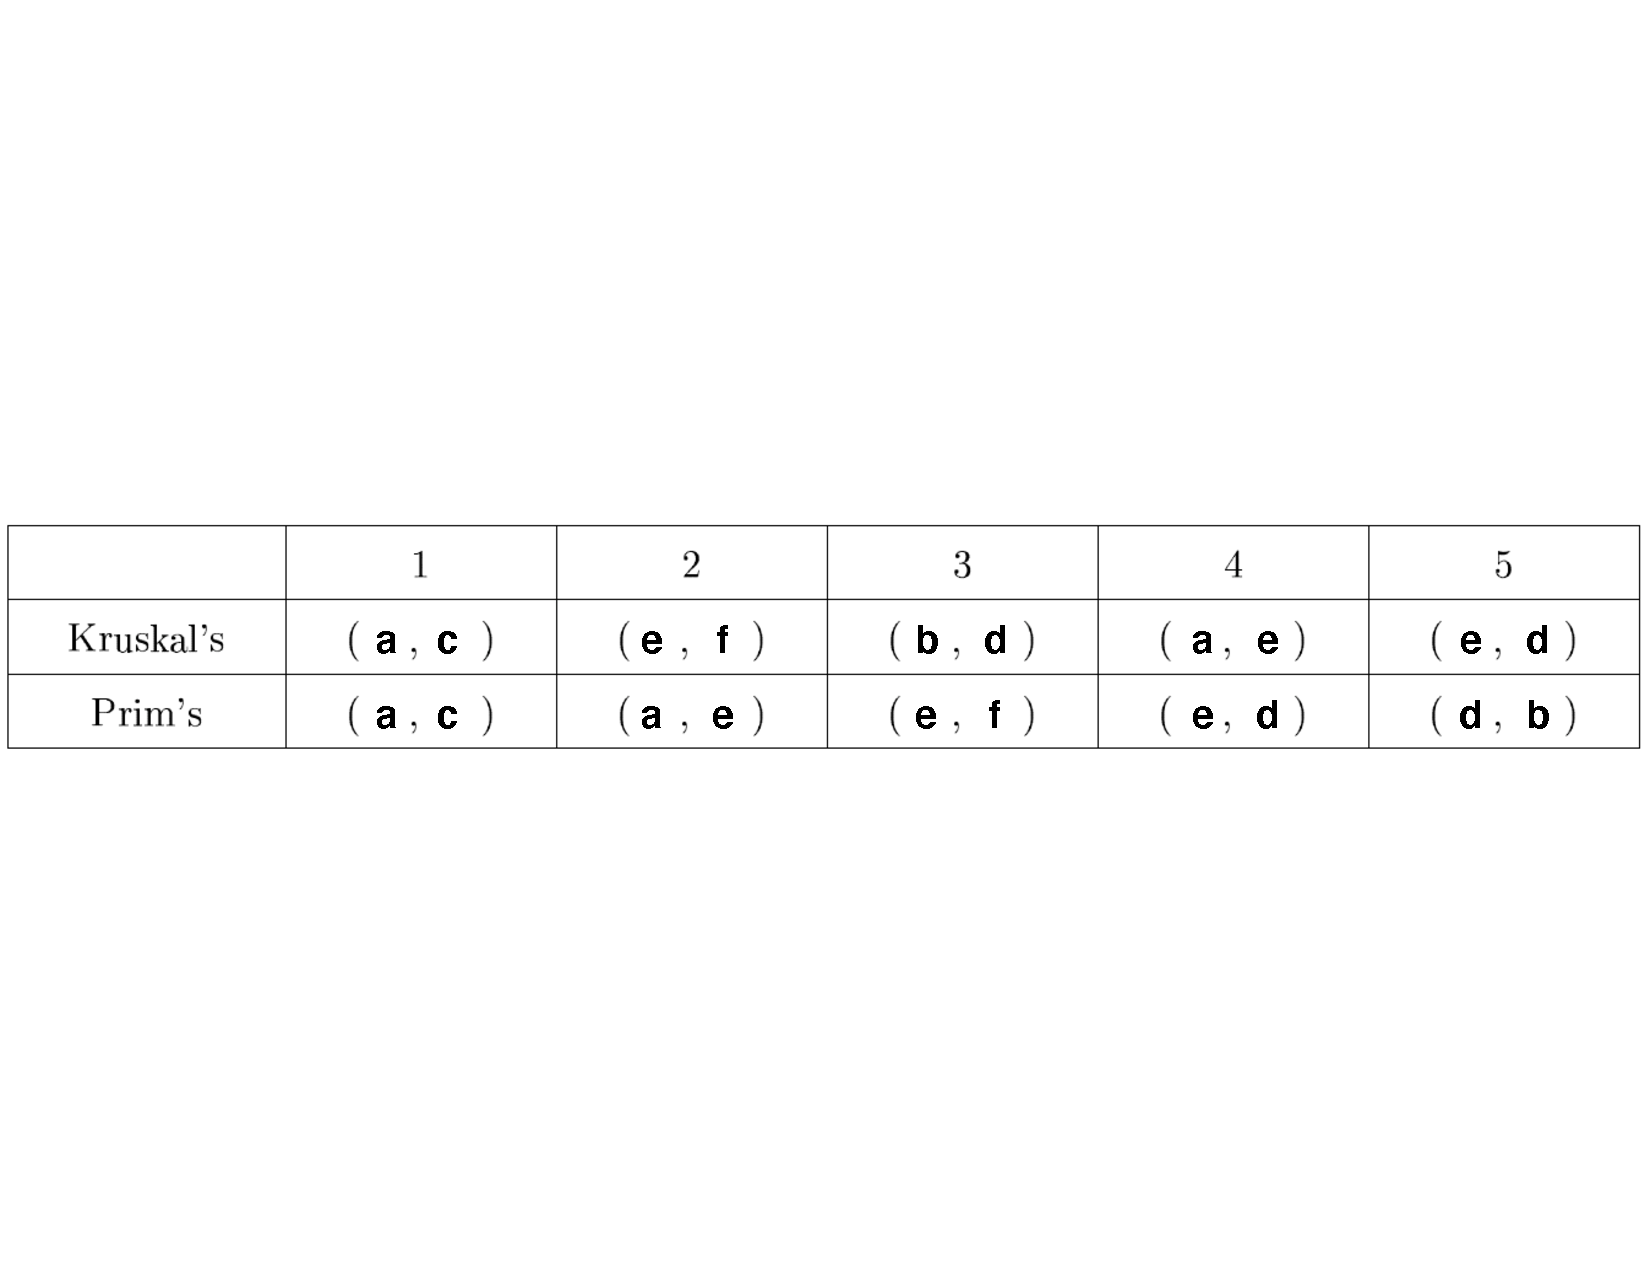
\includegraphics[width=17cm]{MSTb.pdf}
\end{center}
\end{figure}
\newpage
\hrulefill \\

(c) Suppose all edges in a graph $G$ have different edge weights. Show that $G$ has a unique minimum spanning tree.\\
Let us assume we have two MSTs, $T_1$ and $T_2$. Then, consider the edge of minimum weight among all the edges that are contained in exactly on of $T_1$ \emph{or} $T_2$. This edge will only appear in a single tree, say, $T_1$, so let's call it $e_1$. Then, $T_2 \cup \{ e_1 \}$ must contain a cycle, and one of the edges of this cycle, $e_2$, is not in $T_1$.\\
Because $e_2$ is an edge different from $e_1$ and is contained in only one of $T_1$ \emph{or} $T_2$, it must be that $w(e_1) < w(e_2)$. $T$ = $T_2 \cup \{ e_1 \} \backslash \{ e_2 \}$ is a spanning tree. The total weight of $T$ is now smaller than the total weight of $T_2$, but this is a contradiction to our earlier assumption that $T_2$ is a minimum spanning tree.\\
$\therefore$ $G$ has a unique minimum spanning tree if all of the edges in graph $G$ have different costs.

\newpage
\hrulefill \\


\textbf{Problem 2:} (Shortest Paths)\hfill (20 Points)\\

(a) Consider the graph $G$ below.
\begin{figure}[htb]
\begin{center}
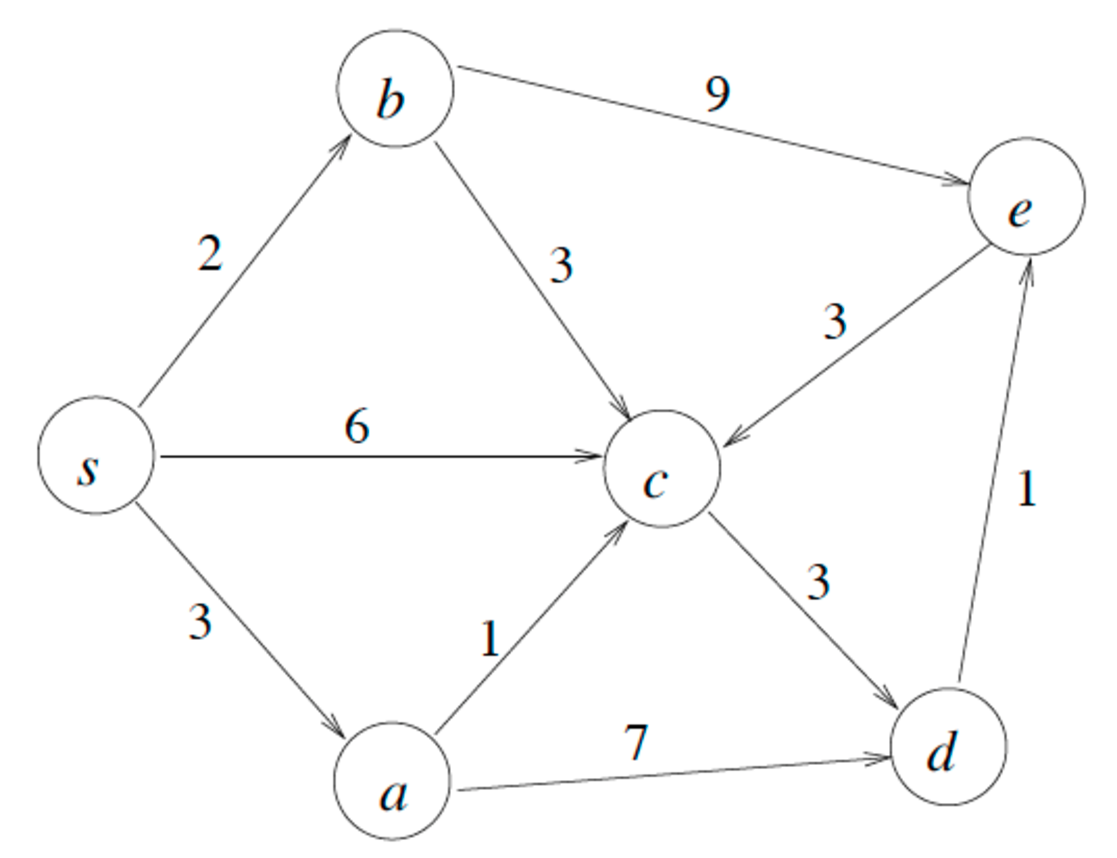
\includegraphics[width=6cm]{SP}
\end{center}
\end{figure}

Show the execution of Dijkstra's algorithm on $G$ by filling out the table below. Assume the source is vertex $s$. You must show the changes in the
d-array at the end of each iteration. Iteration 0 refers to the situation just before the first  iteration of the {\bf while} loop. Also, fill in the vertex that is selected (i.e., extracted from the priority queue) at each iteration.
\begin{figure}[htb]
\begin{center}
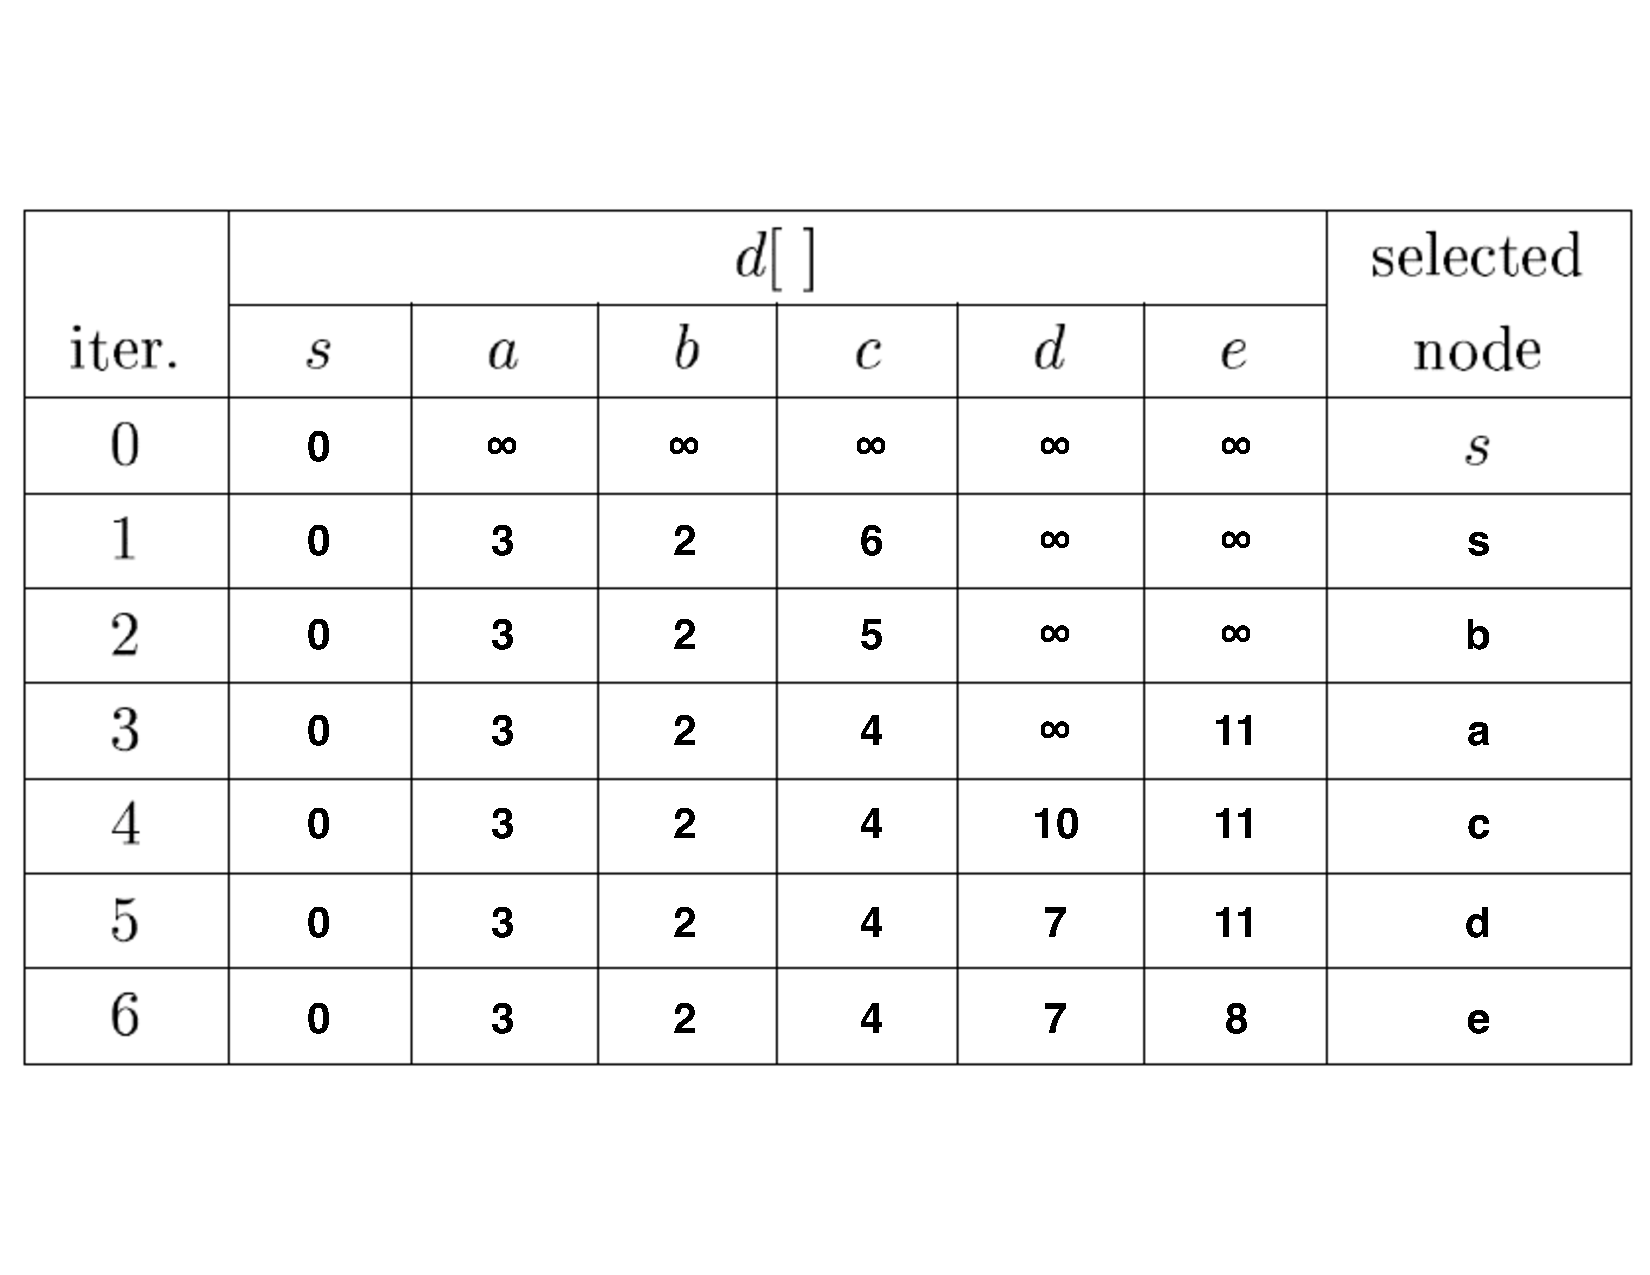
\includegraphics[width=12cm]{SPa.pdf}
\end{center}
\end{figure}

\newpage
\hrulefill \\

(b) Draw a shortest path tree for the graph in (a) with source vertex $s$.
\begin{figure}[htb]
\begin{center}
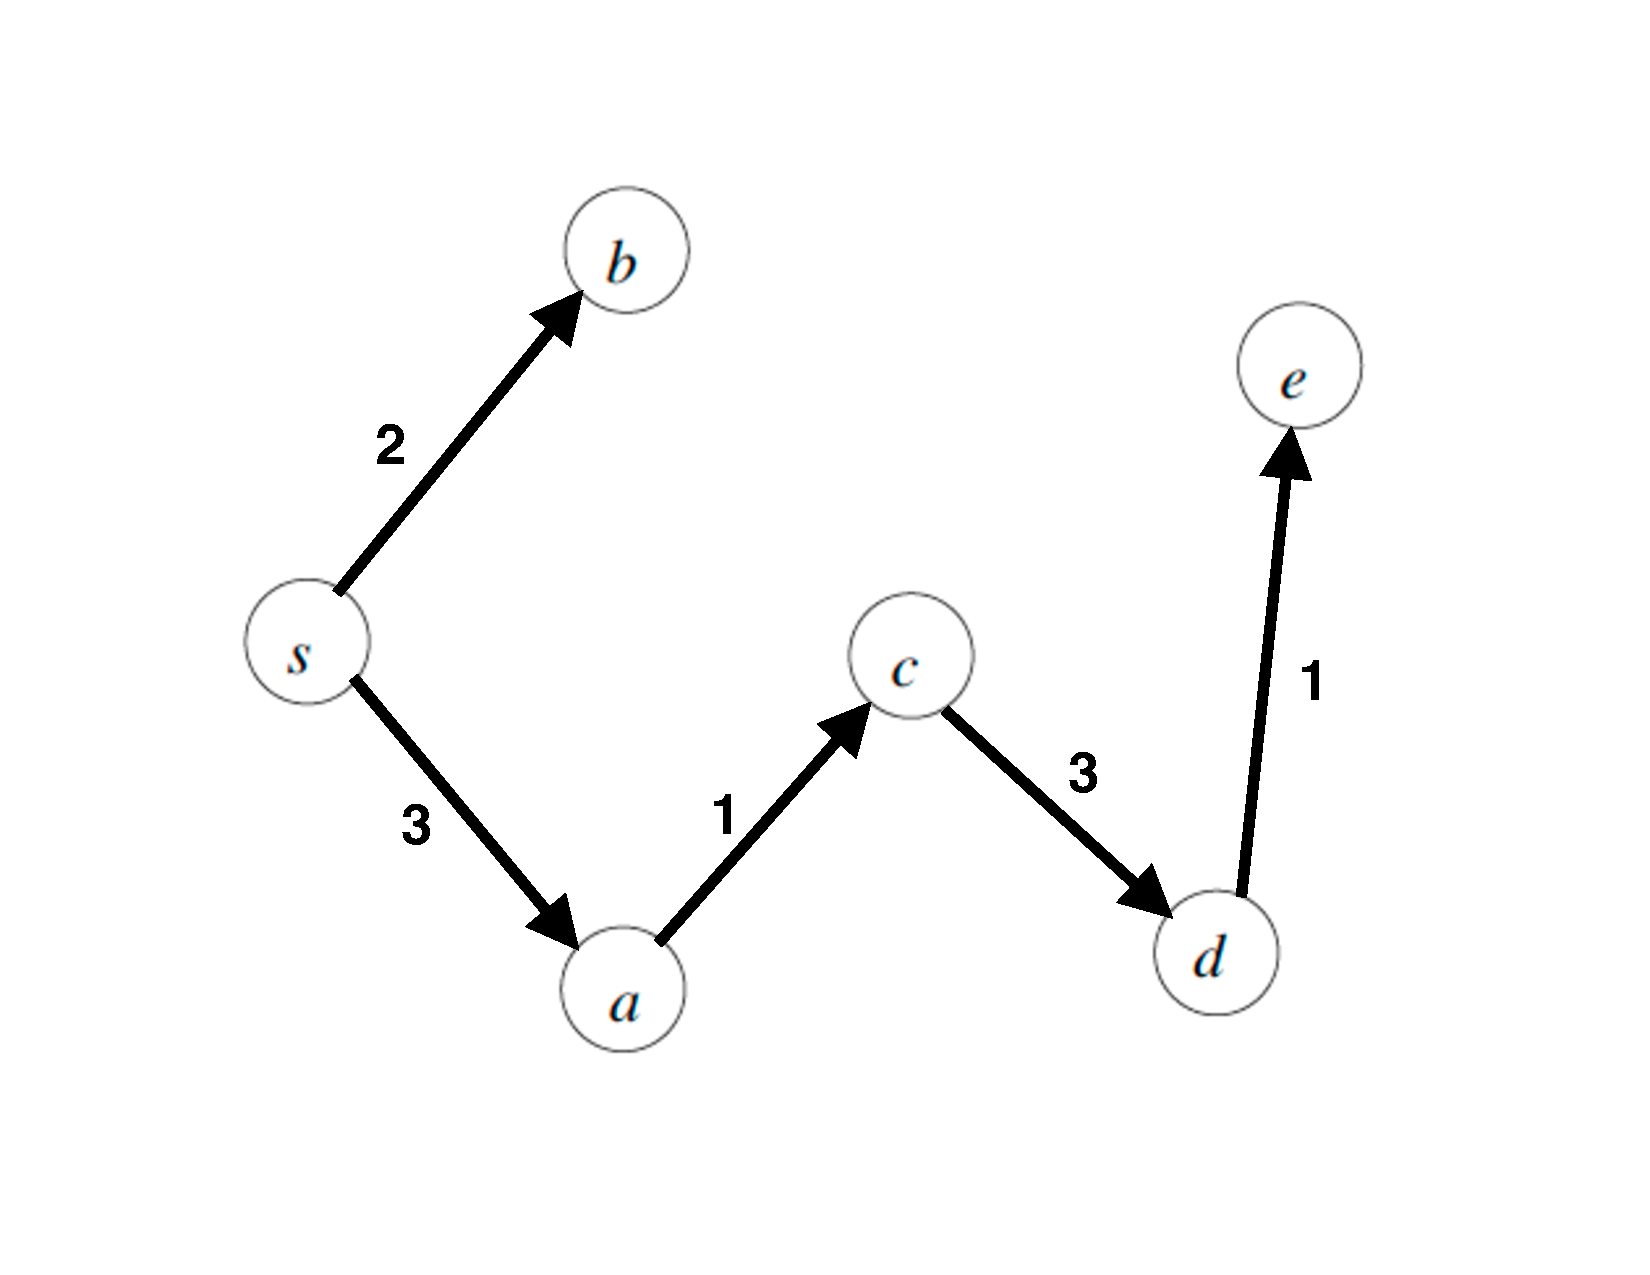
\includegraphics[width=11cm]{SPc}
\end{center}
\end{figure}

(c) Suppose that all edge weights in a given graph $G:=(V,E)$ are NOT negative, and that the shortest path distances in $G$ from a source $s\in V$ to each vertex $v\in V$ are unique. Let $V_k$ denote the vertices in $V$ with the $k$-closest shortest path distances from $s$.\\

\underline{Example:} Let $V=\{s, u, v\}$ and $0, 2, 3$ be the shortest path distances of the vertices  $s, u, v$ from $s$ in $G$ respectively. Then, $s$ is the $1$-closest vertex, $u$ is the $2$-closest vertex, and $v$ is the $3$-closest vertex. Therefore we have $V_1= \{s\}$, $V_2=\{s,u\}$, $V_3=V$.\\ 

Prove by contradiction that a shortest path from the source vertex $s\in V$ to a k-closest vertex $x\in V$ consists only of vertices in $V_k$.\\
\newpage
\hrulefill \\
Let us assume that we have vertexes $V$, we are trying to get to vertex $x \in V$, and our starting vertex is $s \in V$. We also have a shortest path of weight $w$ from $s \in V$ to $x \in V$. Becase it is a shortest path, we know that $w$ is the smallest weight path possible from the two vertexes.\\
Now let us assume that there is another vertex, $V_{k+1}$ that is part of this shortest path from $s$ to $x$. This would mean that the weight of the path would then be $w + e$ where $e$ is the edge weight to the additional vertex $V_{k+1}$. This would also mean that the path from $s$ to $x$ would be the original weight $w$ plus the distance from $x$ to $V_{k+1}$, which is greater than our original shortest path, which is a contradiction of the earlier assumption that the shortest path would include $V_{k+1}$. This also stands with the knowledge that each shortest path from a source vertex to any other vertex is also made up of shortest paths.\\
$\therefore$ A shortest path from the source vertex $s\in V$ to a k-closest vertex $x\in V$ consists only of vertices in $V_k$.

\newpage
\hrulefill \\
\textbf{Problem 3:} (P is Closed under Reverse Complement)\hfill (20 Points)\\

Consider the operation of reverse complement on a language over the alphabet $\{ 0, 1\}$. The reverse complement of a string $x \in \{ 0, 1 \}^*$ of length $n$ is a string $y \in \{ 0, 1 \}^*$ of the same length such that $y_k = 1 - x_{n-k+1}$ for $k = 1, 2, ..., n$, where $y_k$ is the bit at index $k$ of string $y$. Let $\overline{x}$ denote the reverse complement of string $x$. For example, if $x = 011101$, then $\overline{x} = 010001$. Note that $\overline{x}$ is obtained from  $x$ by reversing its bit sequence
and complementing each bit (changing $1$ to $0$ and $0$ to $1$). Let $L$ be a language over the alphabet $\{ 0, 1\}$. The reverse complement of $L$ is defined as \\

$\overline{L} = \{ \overline{x} : x \in L \}$. \\

Show that if $L$ is in P, then $\overline{L}$ is also in P. Note that the reverse complement of $L$ is not related to the set complement of $L$. Your algorithm takes as input a binary string in $\{ 0, 1 \}^*$.
\begin{algorithm}[H]
    \Fn(){ReverseComplement}{
    \KwIn{A binary string $x$ in $\{ 0, 1 \}^*$}
    \SetAlgoLined
    \SetNoFillComment
    \DontPrintSemicolon
        Let $y$ be a new string of the same size of $x$, size $n$\\
        \For{$k = 1$ to $n$} {
            $y_k = x_{k - n + 1}$
        }
        return $y$
    }
    \end{algorithm}
For this algorithm, we take in an input string $x$ and, through the given formula of $y_k = x_{k - n + 1}$, convert is into a "Reverse Complement" $y$ of the original input string $x$. It is iterating through the original input size of $n$ exactly once, from 1 to $k$ where $k$ is set equal to $n$. Because of this, it is able to produce output in $O(n^k)$ time where $k$ = 1, so this problem is $O(n^1)$.\\
$\therefore \overline{L}$ is in $P$.
\newpage
\hrulefill \\
\textbf{Problem 4:} (String Transformation is in NP)\hfill (20 Points)\\

A string $x \in \{ 0, 1 \}^*$ is transformed into another string $y$ by a sequence of operations of two types. Let $x$ be a string of $n$ bits, indexed from $1$ to $n$, where $x_{i,j}$ denotes a substring of $x$, consisting of consecutive bits from index $i$ to index $j$ in the same order, with $1 \leq i \leq j \leq n$. Let $xyz$ denote the concatenation of strings $x$, $y$, and $z$. An inversion operation $r(i,j)$ turns string $x$ into $x_{1, i-1} \overline{x_{i, j}} x_{j+1, n}$, with $1 \leq i \leq j \leq n$, where $\overline{x_{i, j}}$ is the reverse complement of $x_{i, j}$ (see problem 3). A deletion operation $d(i,j)$ turns string $x$ into $x_{1, i-1} x_{j+1, n}$. For example, an inversion operation $r(3, 6)$ transforms string $11011100$ into string $11000100$ ($x_{3, 6} = 0111$, $\overline{x_{3, 6}} = 0001$), which is further transformed into string $100100$ by a deletion operation $d(2, 3)$.
Show that the problem of deciding whether a string can be
transformed into another string by a sequence of at most $k$ operations of
substring deletions and inversions is in NP. Specifically, the problem is defined
as the formal language \\

$\textrm{ST} = \{ <x, y, k>: \textrm{there exists a sequence of at most}\; k \; \textrm{operations}$

$\qquad \qquad \textrm{of deletions and inversions to transform binary strings}\; x\; \textrm{into}\; y\; \}$. \\

Show that ST is in NP. Note that your algorithm takes two types of input: one type is an ordinary input including two strings $x$ and $y$ along with an integer $k$, and the other is a certificate.\\
\newpage
\hrulefill \\
In order for ST to be in NP, there needs to be an efficient polynomial time certifier that can effectivey run a specific instance with the correct certificate. We are given a string $x$ of $n$ bits, an "end result" $y$, an integer $k$, and a certificate $c$. The language is defined as\\ L $= \{ x \in \{0,1\}^*, y \in \{0,1\}^*, k:$ there exists a certificate, $c \in \{0,1\}^*$, with $|c| = O(|x|^c)$ such that StringTransformation(x,y,k,c) $= 1 \}$ In essence, $c$ is the certificate that will be the most optimal choice to operate on $x$ with either deletion or reverse complement polynomial algorithms to get one step closer to $y$. This can be done at most $k$ times to decide if $x$ can be transformed into $y$.\\
\newpage
\hrulefill \\
\begin{algorithm}[H]
    \Fn(){StringTransformation}{
    \KwIn{A string $x$ of $n$ bits, an "end result" string $y$, integer $k$, and certificate $c$}
    \SetAlgoLined
    \SetNoFillComment
    \DontPrintSemicolon
        \CommentSty{Not possible in the number of total runs we've done}\\
        \If{number of runs $>$ k} {
            return false
        }

        \If{$x$ == $y$} {
            return true
        }
        \If{$x$ is smaller than $y$} {
            return false
        }

        \CommentSty{We know that we need to perform delete operations to get it closer}\\
        \If{size of $x >$ size of $c$} {
            \For{i = 0 to size of $x$} {
                \For{j = 0 to size of $x$} {
                    \CommentSty{Assuming non-destructive r and d methods}\\
                    \If{result of d(i, j) == $c$} {
                        return true
                    }
                }
            }
        }

        \CommentSty{This is in the instance where we are the same size, and now we need to perform reverse complement operations on input}\\
        \For{i = 0 to size of $x$} {
            \For{j = 0 to size of $x$} {
                \CommentSty{Assuming non-destructive r and d methods}\\
                \If{result of r(i, j) == $c$} {
                    return true
                }
            }
        }
    }
    \end{algorithm}
\newpage
\hrulefill \\
The overall runtime of this algorithm can be justified as being 2 runs on the input size of $n$ meaning a polynomial runtime of $n^2$ as well as mutiplying polynomial time operations of $r(i, j)$ and $d(i, j)$, meaning a total runtime of $n^2 * n^k$ or $n^{2k}$ which is still within a polynomial runtime. Additionally, we know that the certificate input string will yield the next best decision of either a $d(i, j)$ or an $r(i, j)$. Because we know we have an algorithm with an efficient polynomial certifier, we can say that ST is in NP.
\newpage
\hrulefill \\
\textbf{Problem 5:} (Restricted CNF-SAT is in P)\hfill (20 Points)\\

A boolean formula in conjunctive normal form, or CNF, is expressed as an AND of clauses, each of which is the OR of one or more literals. A restricted CNF formula meets the following requirements. For every clause with two or more literals in the formula, if the clause contain literal $x$, then no clause can contain $\neg x$, and if it contain $\neg x$, then no clause can contain $x$. If any clause with only one literal contains $x$ or $\neg x$, then this literal cannot occur in any clause with two or more literals. For example, the boolean formulas, \\

$(x_1 \vee \neg x_2 ) \wedge (\neg x_3 \vee x_4 \vee x_5 ) \wedge x_6 \wedge \neg x_6$, and

$(x_1 \vee \neg x_2 ) \wedge (\neg x_3 \vee x_4 \vee x_5 ) \wedge x_6 \wedge \neg x_7$, \\

meet the requirements, and the following formulas do not, \\

$(x_1 \vee \neg x_2 ) \wedge (\neg x_3 \vee x_4 \vee x_5 ) \wedge x_2$, and

$(x_1 \vee \neg x_2 ) \wedge (\neg x_1 \vee x_2 \vee x_5 )$. \\

Show that the problem of deciding whether a restricted boolean formula in CNF is satisfiable is in P. Specifically, the problem is defined as the formal language \\

$\textrm{RES-CNF} = \{ <\theta> : \theta \; \textrm{is a satisfiable restricted boolean formula in CNF} \}$. \\

Show that RES-CNF is in P. Note that input to your algorithm is a restricted boolean formula in CNF.\\
\newpage
\hrulefill \\
\begin{algorithm}[H]
    \Fn(){RES-CNF}{
    \KwIn{A restricted boolean formula $f$ in CNF}
    \SetAlgoLined
    \SetNoFillComment
    \DontPrintSemicolon
        Let $SingleLiterals$ be a list to hold literals by themselves, meaning a single literal in a clause\\
        \For{$i$ = 0 to input string $f$ length} {
            \CommentSty{If $i$ is a literal in the form $x_n$ and is single, as explained above}\\
            \If{$i$ is complete clause and SingleLiteral($i$)} {
                Add $i$ to SingleLiterals
            }
        }

        \For{$j$ = 0 to length of SingleLiterals} {
            \For{$k$ = 0 to length of SingleLiterals} {
                \CommentSty{If we have a single literal in a clause with a $\neg$ counterpart, i.e. $x_6$ and $\neg x_6$}\\
                \If{Input[i] == $\neg$Input[j]}{
                    return false
                }
            }
        }

        return true
    }
    \end{algorithm}
\bigskip
This algorithm will determine if an expression is satisfiable in the RES-CNF form given. We know that an expression will always be able to evalutate to TRUE with varied inputs for the values of $x_1$ to $x_n$ except in the case where there are two standalone literals that are the negation of the other, such as in the case of $x_6 \wedge \neg x_6$ standalone clauses. This algorithm will go through the input CNF and find the clauses which are a standalone literal, which can be found in $O(n)$ time, then it iterates through the list of these standalone clauses in $O(n^2)$ time, leading to an overall runtime of $n^2 + n$ or a big O of $O(n^2)$ which is $O(n^k)$ where $k$ is 2. Because of this, we can say that deciding whether a RES-CNF is satisfiable is in P.
\end{document}